% Options for packages loaded elsewhere
\PassOptionsToPackage{unicode}{hyperref}
\PassOptionsToPackage{hyphens}{url}
%
\documentclass[
  11pt,
]{article}
\usepackage{amsmath,amssymb}
\usepackage{iftex}
\ifPDFTeX
  \usepackage[T1]{fontenc}
  \usepackage[utf8]{inputenc}
  \usepackage{textcomp} % provide euro and other symbols
\else % if luatex or xetex
  \usepackage{unicode-math} % this also loads fontspec
  \defaultfontfeatures{Scale=MatchLowercase}
  \defaultfontfeatures[\rmfamily]{Ligatures=TeX,Scale=1}
\fi
\usepackage{lmodern}
\ifPDFTeX\else
  % xetex/luatex font selection
\fi
% Use upquote if available, for straight quotes in verbatim environments
\IfFileExists{upquote.sty}{\usepackage{upquote}}{}
\IfFileExists{microtype.sty}{% use microtype if available
  \usepackage[]{microtype}
  \UseMicrotypeSet[protrusion]{basicmath} % disable protrusion for tt fonts
}{}
\makeatletter
\@ifundefined{KOMAClassName}{% if non-KOMA class
  \IfFileExists{parskip.sty}{%
    \usepackage{parskip}
  }{% else
    \setlength{\parindent}{0pt}
    \setlength{\parskip}{6pt plus 2pt minus 1pt}}
}{% if KOMA class
  \KOMAoptions{parskip=half}}
\makeatother
\usepackage{xcolor}
\usepackage[letterpaper,margin=2.5cm]{geometry}
\usepackage{longtable,booktabs,array}
\usepackage{calc} % for calculating minipage widths
% Correct order of tables after \paragraph or \subparagraph
\usepackage{etoolbox}
\makeatletter
\patchcmd\longtable{\par}{\if@noskipsec\mbox{}\fi\par}{}{}
\makeatother
% Allow footnotes in longtable head/foot
\IfFileExists{footnotehyper.sty}{\usepackage{footnotehyper}}{\usepackage{footnote}}
\makesavenoteenv{longtable}
\usepackage{graphicx}
\makeatletter
\def\maxwidth{\ifdim\Gin@nat@width>\linewidth\linewidth\else\Gin@nat@width\fi}
\def\maxheight{\ifdim\Gin@nat@height>\textheight\textheight\else\Gin@nat@height\fi}
\makeatother
% Scale images if necessary, so that they will not overflow the page
% margins by default, and it is still possible to overwrite the defaults
% using explicit options in \includegraphics[width, height, ...]{}
\setkeys{Gin}{width=\maxwidth,height=\maxheight,keepaspectratio}
% Set default figure placement to htbp
\makeatletter
\def\fps@figure{htbp}
\makeatother
\setlength{\emergencystretch}{3em} % prevent overfull lines
\providecommand{\tightlist}{%
  \setlength{\itemsep}{0pt}\setlength{\parskip}{0pt}}
\setcounter{secnumdepth}{-\maxdimen} % remove section numbering
\ifLuaTeX
\usepackage[bidi=basic]{babel}
\else
\usepackage[bidi=default]{babel}
\fi
\babelprovide[main,import]{spanish}
% get rid of language-specific shorthands (see #6817):
\let\LanguageShortHands\languageshorthands
\def\languageshorthands#1{}
% Ajustes de calidad editorial para los boletines IES.
% Se incluyen con: pandoc --include-in-header=assets/editorial.tex
% Nota: pandoc ya carga `microtype` automáticamente si está disponible,
% por eso aquí solo se afinan los pies de figura.
\usepackage{caption}     % control de los pies de figura
\captionsetup{font=small, labelfont=bf}
\ifLuaTeX
  \usepackage{selnolig}  % disable illegal ligatures
\fi
\IfFileExists{bookmark.sty}{\usepackage{bookmark}}{\usepackage{hyperref}}
\IfFileExists{xurl.sty}{\usepackage{xurl}}{} % add URL line breaks if available
\urlstyle{same}
\hypersetup{
  pdflang={es},
  hidelinks,
  pdfcreator={LaTeX via pandoc}}

\author{}
\date{}

\begin{document}

\hypertarget{termodinuxe1mica-financiera-03-wall-street-y-capex-en-ia}{%
\section{TERMODINÁMICA FINANCIERA 03: Wall Street y CapEx en
IA}\label{termodinuxe1mica-financiera-03-wall-street-y-capex-en-ia}}

\textbf{Edición Especial:} La Rotación de Wall Street y el Colapso de la
Activación sin Flujo

\textbf{Caso:} Exceso de CAPEX en IA, Rotación de Capital y el Mercado
de Bonos (CNBC / Jim Cramer - Julio 2026)

https://www.cnbc.com/2026/07/28/jim-cramer-wall-street-fleeing-ai-trade-buying-these-stocks.html

\begin{center}\rule{0.5\linewidth}{0.5pt}\end{center}

\hypertarget{titular-y-resumen-ejecutivo}{%
\subsection{1. Titular y Resumen
Ejecutivo}\label{titular-y-resumen-ejecutivo}}

\textbf{Titular:} Wall Street Huye de la ``Falsa Restricción'': El
Capital Migra del \(I\) Inflado al Throughput (\(T\)) Real.

\textbf{Resumen Ejecutivo:}

El éxodo de capital desde las Megacaps tecnológicas hiperapalancadas
hacia sectores tradicionales no es una simple ``rotación defensiva'' ni
una aversión al riesgo sectorial. Representa el reconocimiento del
sistema financiero de que la restricción global ha mutado. La
acumulación masiva de infraestructura de IA (GPUs, servidores)
financiada con deuda ha generado un exceso de \textbf{Inventario (\(I\))
subutilizado (solo \textasciitilde5\% de uso real)}. Con el mercado de
bonos exigiendo rendimientos reales y el costo del capital elevado, Wall
Street abandona las métricas de eficiencia local y la especulación de
valoración para subordinarse al flujo de caja (\(T\)) inmediato y
desapalancado.

\begin{center}\rule{0.5\linewidth}{0.5pt}\end{center}

\hypertarget{diagnuxf3stico-del-sistema-seguxfan-toc}{%
\subsection{2. Diagnóstico del Sistema según
TOC}\label{diagnuxf3stico-del-sistema-seguxfan-toc}}

\begin{itemize}
\tightlist
\item
  \textbf{El Sistema bajo Análisis:} La red global de asignación de
  capital (Renta Variable vs.~Mercado de Deuda Corporativa y Bonos
  Sovereign).
\item
  \textbf{La Restricción del Sistema (Cuello de Botella):} La
  \textbf{Capacidad de Monetización y Generación de Flujo de Caja Real
  (\(T\))}. La restricción ya no es la capacidad física de cómputo o el
  acceso a chips, sino la integración efectiva de la tecnología en la
  economía real para producir liquidez neta.
\end{itemize}

\begin{figure}
\centering
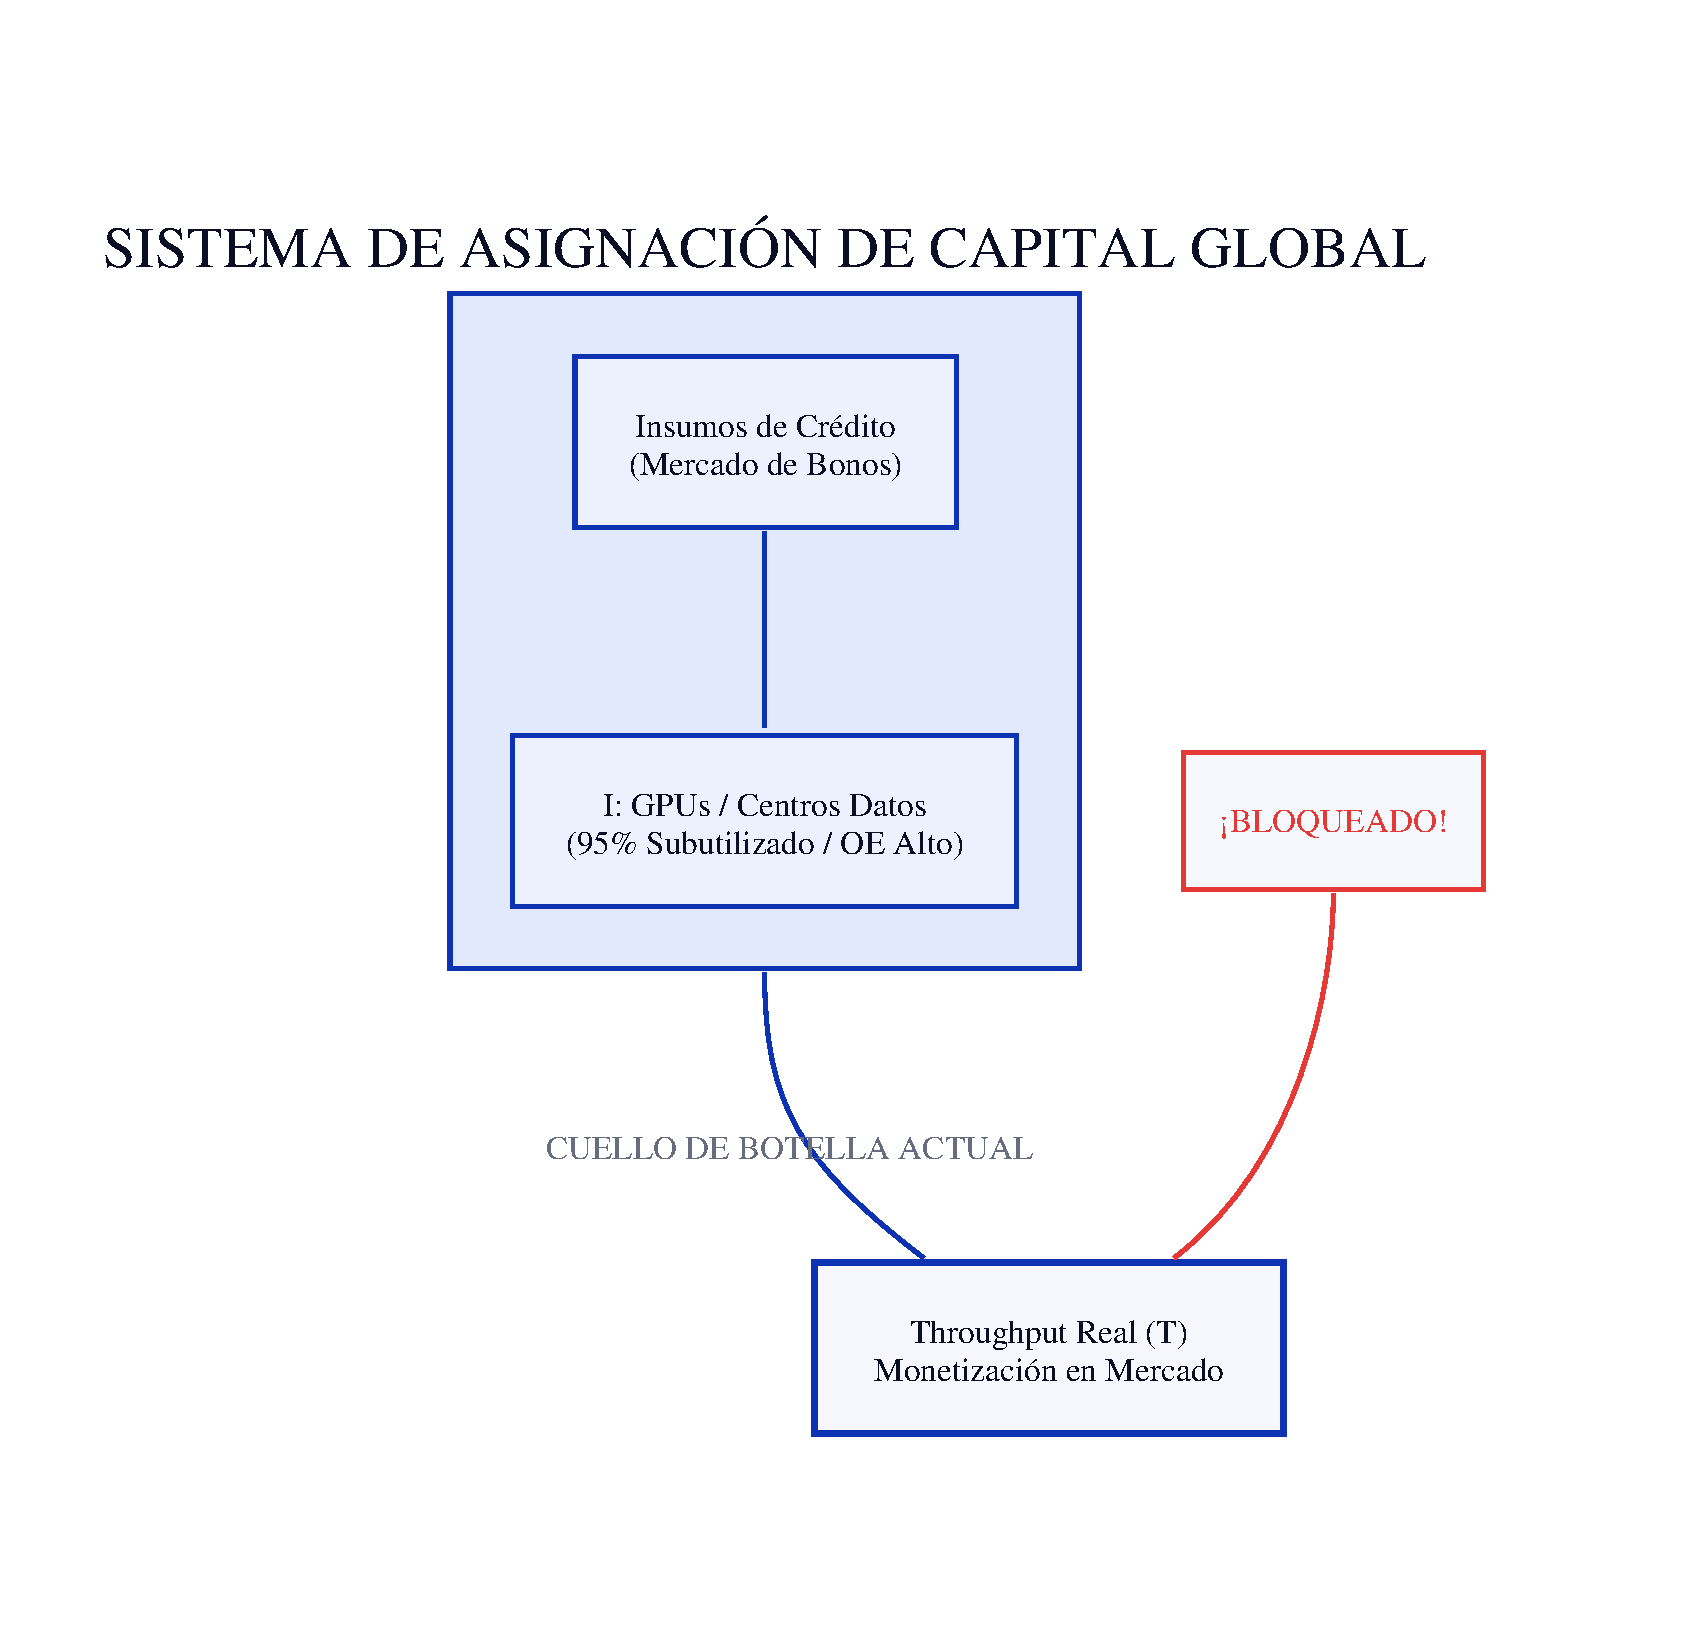
\includegraphics{Diagramas/flujo-sistema-capital.pdf}
\caption{Sistema de Asignación de Capital Global y su Cuello de Botella}
\end{figure}

\hypertarget{impacto-en-los-3-paruxe1metros-clave-de-goldratt}{%
\subsubsection{Impacto en los 3 Parámetros Clave de
Goldratt}\label{impacto-en-los-3-paruxe1metros-clave-de-goldratt}}

\begin{itemize}
\tightlist
\item
  \textbf{Throughput (\(T\)):} Estancado en el sector tecnológico. El
  valor de los tokens y el costo de la hora de GPU caen en los mercados
  secundarios mientras las ventas finales a clientes corporativos tardan
  en materializarse. Por el contrario, los sectores tradicionales
  (bancos, retail, salud) mantienen un \(T\) recurrente e instantáneo.
\item
  \textbf{Inversión / Inventario (\(I\)):} Hiperextendido. Miles de
  millones de dólares en hardware de IA comprados a precios inflados
  (\$30,000--\$40,000 USD por GPU) actúan como un \textbf{Inventario
  congelado} con una tasa de depreciación y obsolescencia técnica
  devastadora (18 a 24 meses).
\item
  \textbf{Gasto de Operación (\(OE\)):} Disparado. El costo del servicio
  de la deuda emitido en el mercado de bonos, sumado a los costos fijos
  de energía, mantenimiento, licencias y refrigeración líquida para
  mantener activo el 95\% del hardware subutilizado, está erosionando el
  margen neto.
\end{itemize}

\begin{center}\rule{0.5\linewidth}{0.5pt}\end{center}

\hypertarget{herramienta-de-procesos-de-pensamiento-nube-de-evaporaciuxf3n-evaporating-cloud}{%
\subsubsection{Herramienta de Procesos de Pensamiento: Nube de
Evaporación (Evaporating
Cloud)}\label{herramienta-de-procesos-de-pensamiento-nube-de-evaporaciuxf3n-evaporating-cloud}}

\begin{figure}
\centering
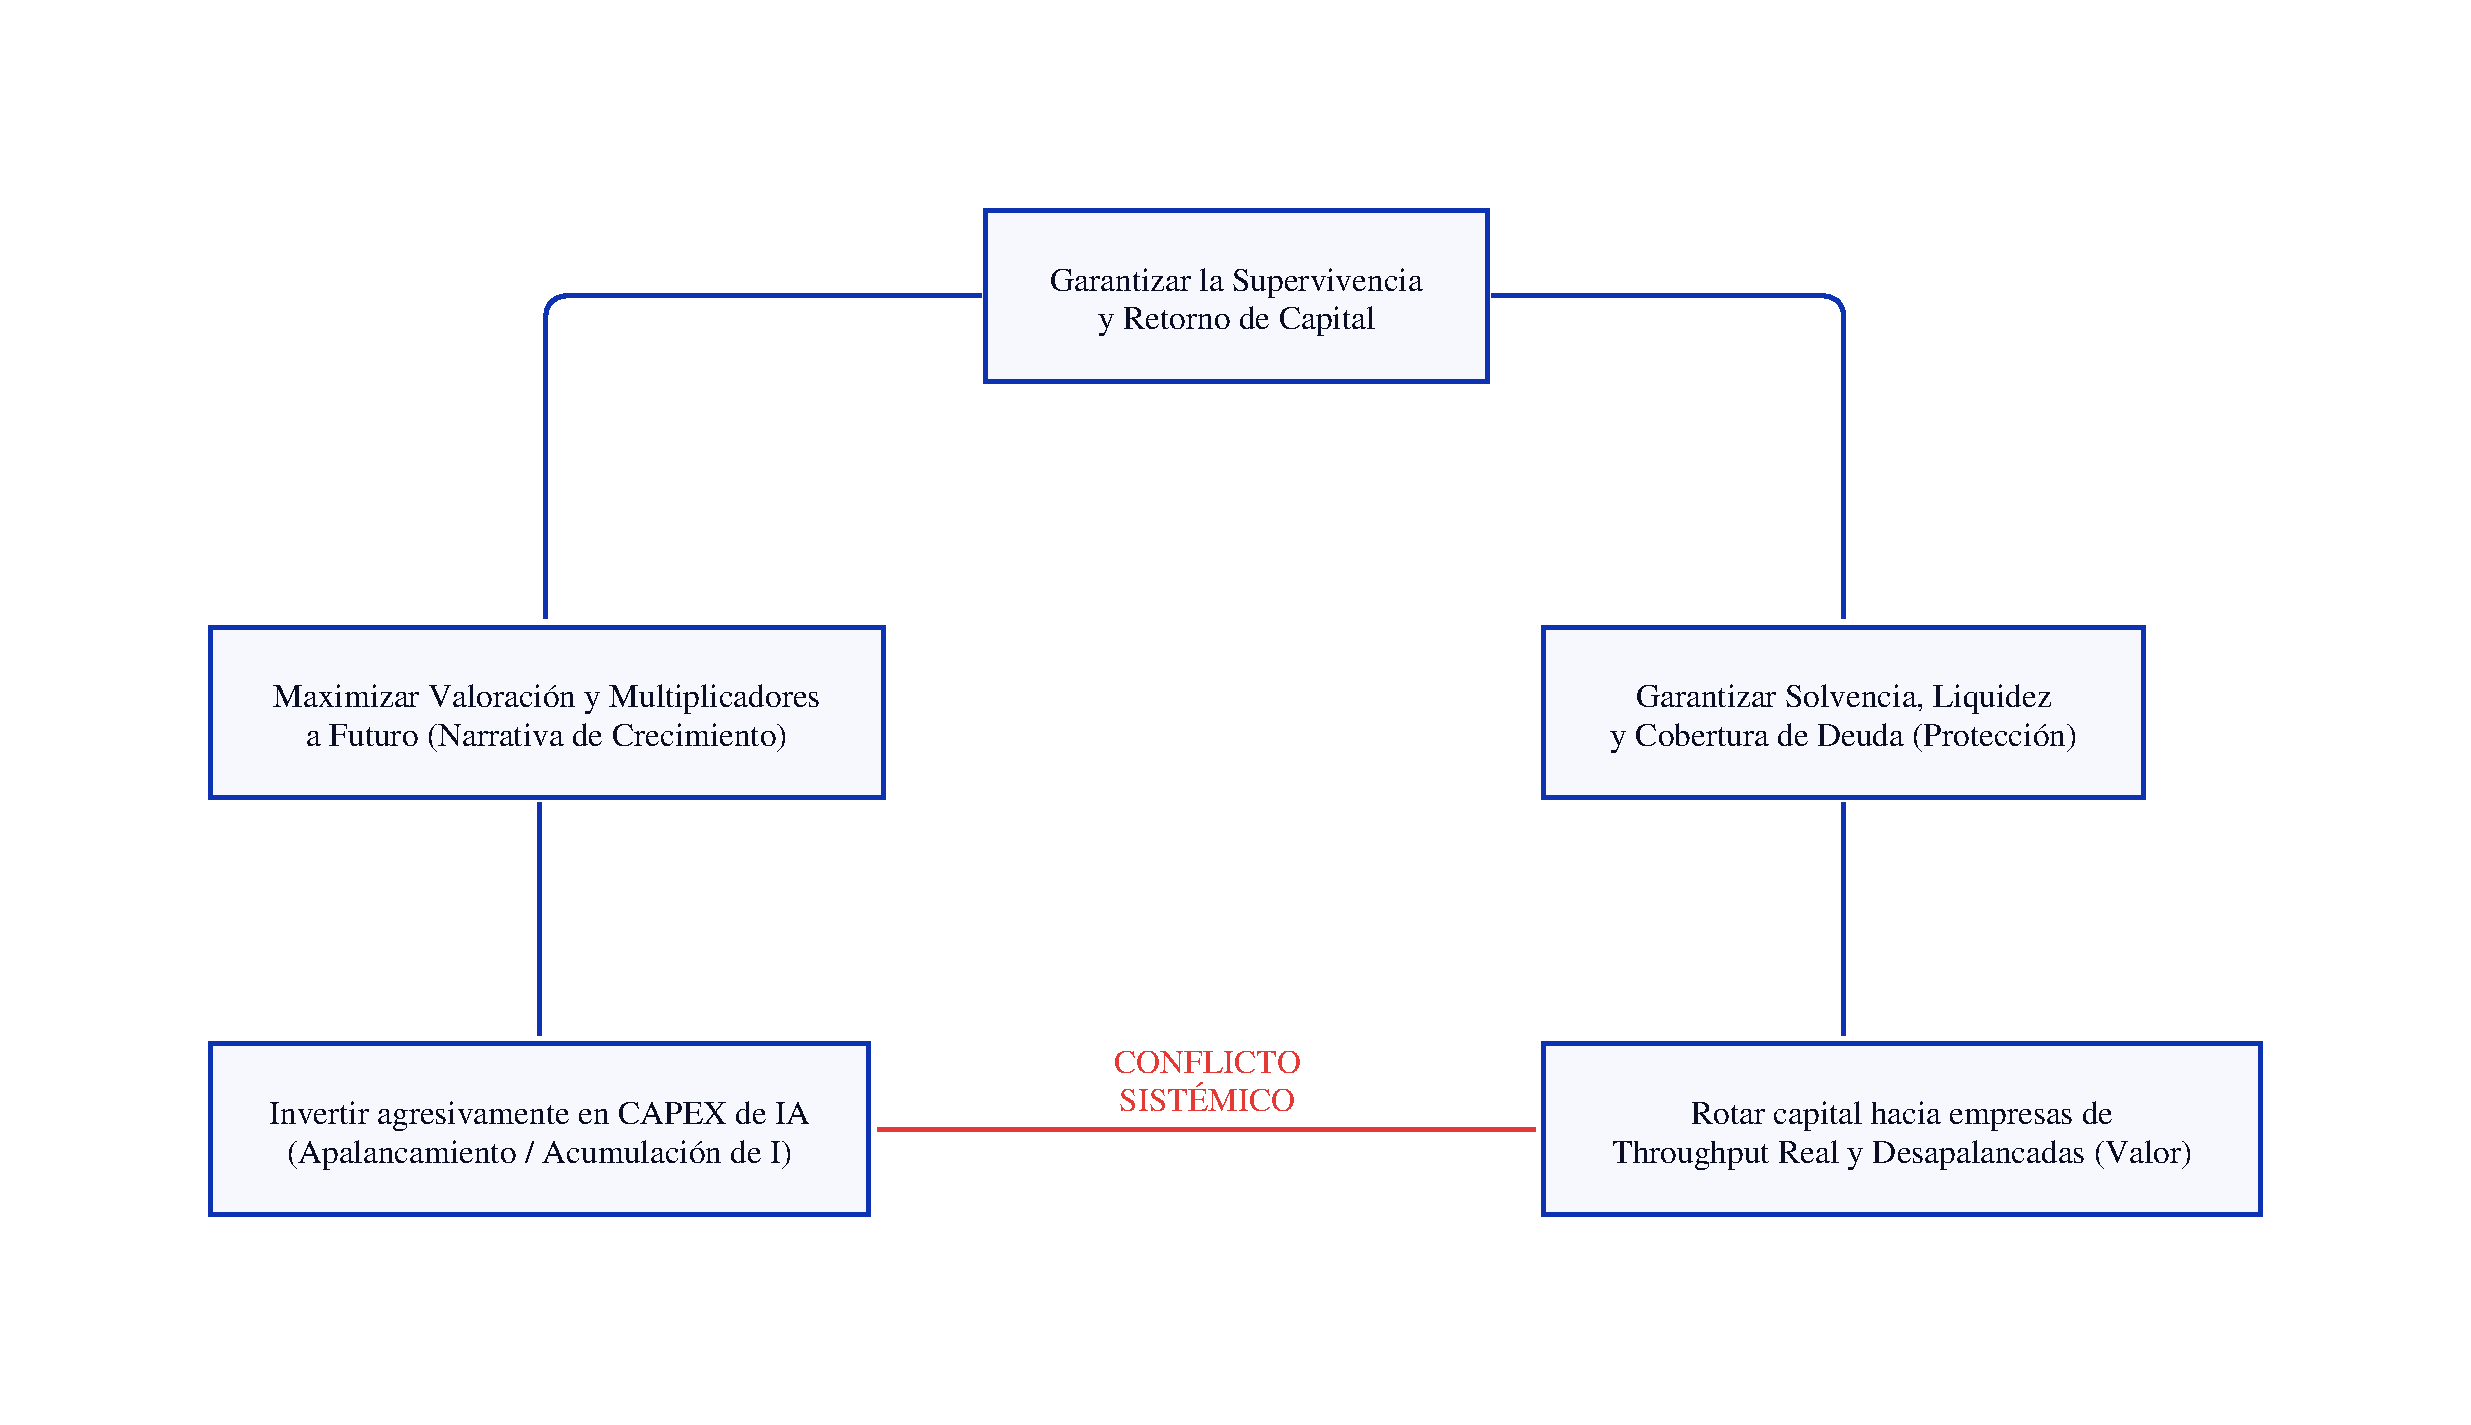
\includegraphics{Diagramas/nube-evaporacion-capex.pdf}
\caption{Nube de Evaporación del Conflicto: CAPEX en IA vs.~Throughput
Real}
\end{figure}

\begin{itemize}
\tightlist
\item
  \textbf{El Supuesto Falso a Evaporar:} Se asumía la premisa de que
  \emph{``Incrementar la Inversión (\(I\)) en infraestructura
  tecnológica se traduciría automáticamente en Throughput (\(T\)) a
  velocidad infinita''}. La exigencia del mercado de bonos rompe este
  supuesto, forzando la migración del capital hacia {[}D'{]}.
\end{itemize}

\begin{center}\rule{0.5\linewidth}{0.5pt}\end{center}

\hypertarget{dicotomuxeda-clave-1-contabilidad-de-costos-tradicional-vs.-contabilidad-del-throughput-ta}{%
\subsection{3. Dicotomía Clave 1: Contabilidad de Costos Tradicional
vs.~Contabilidad del Throughput
(TA)}\label{dicotomuxeda-clave-1-contabilidad-de-costos-tradicional-vs.-contabilidad-del-throughput-ta}}

\begin{longtable}[]{@{}
  >{\raggedright\arraybackslash}p{(\columnwidth - 4\tabcolsep) * \real{0.3333}}
  >{\raggedright\arraybackslash}p{(\columnwidth - 4\tabcolsep) * \real{0.3333}}
  >{\raggedright\arraybackslash}p{(\columnwidth - 4\tabcolsep) * \real{0.3333}}@{}}
\toprule\noalign{}
\begin{minipage}[b]{\linewidth}\raggedright
Variable
\end{minipage} & \begin{minipage}[b]{\linewidth}\raggedright
Contabilidad de Costos Tradicional (GAAP/IFRS)
\end{minipage} & \begin{minipage}[b]{\linewidth}\raggedright
Contabilidad del Throughput (TOC / TA)
\end{minipage} \\
\midrule\noalign{}
\endhead
\bottomrule\noalign{}
\endlastfoot
\textbf{Tratamiento del Hardware / GPUs} & Es un \textbf{Activo Fijo
(CAPEX)}. Se activa en el balance y se amortiza gradualmente a 3--5
años, simulando solvencia y capitalización. & Es \textbf{Inventario
(\(I\)) y Gasto (\(OE\))}. Al estar utilizado al \textasciitilde5\%, es
dinero atrapado que consume recursos (electricidad, intereses) sin
generar retorno. \\
\textbf{Métrica de Eficiencia} & \textbf{Eficiencia Local / Uso de
Capacidad.} Busca activar las máquinas/módulos para ``repartir los
costos fijos'', generando sobreproducción de cómputo. & \textbf{Tasa de
Flujo del Sistema.} La activación sin Throughput es un error
catastrófico (\emph{Activación \(\neq\) Productividad}). Si el chip no
produce \(T\), operarlo solo incrementa \(OE\). \\
\textbf{Evaluación del Apalancamiento} & ``Deuda buena'' que financia el
crecimiento operativo e incrementa el EBITDA proyectado a largo plazo. &
\textbf{Riesgo Sistémico de Ahogamiento.} La deuda incrementa el \(OE\)
de forma rígida. Si el \(T\) no llega antes del vencimiento del bono, el
\(I\) se castiga (\emph{write-off}). \\
\end{longtable}

\begin{center}\rule{0.5\linewidth}{0.5pt}\end{center}

\hypertarget{dicotomuxeda-clave-2-teoruxeda-monetaria-moderna-mmt-vs.-teoruxeda-de-restricciones-toc}{%
\subsection{4. Dicotomía Clave 2: Teoría Monetaria Moderna (MMT)
vs.~Teoría de Restricciones
(TOC)}\label{dicotomuxeda-clave-2-teoruxeda-monetaria-moderna-mmt-vs.-teoruxeda-de-restricciones-toc}}

\hypertarget{visiuxf3n-de-la-mmt-modern-monetary-theory}{%
\subsubsection{Visión de la MMT (Modern Monetary
Theory)}\label{visiuxf3n-de-la-mmt-modern-monetary-theory}}

\begin{itemize}
\tightlist
\item
  \textbf{Premisa:} La restricción financiera nominal no existe mientras
  exista capacidad de emisión o acceso al crédito respaldado
  institucionalmente. Los grandes déficit de capital e inversiones en
  infraestructura de vanguardia (como la IA) son deseables y sostenibles
  mediante expansión crediticia o apoyo estatal, ya que crean activos
  productivos en los balances sectoriales.
\item
  \textbf{Interpretación de la Noticia:} Consideraría que la salida del
  \emph{trade} de IA es un reajuste temporal de liquidez en los mercados
  secundarios y una mala asignación de riesgo crediticio privado que
  requiere estabilización o refinanciación para evitar un evento
  deflacionario.
\end{itemize}

\hypertarget{visiuxf3n-de-la-toc-theory-of-constraints}{%
\subsubsection{Visión de la TOC (Theory of
Constraints)}\label{visiuxf3n-de-la-toc-theory-of-constraints}}

\begin{itemize}
\tightlist
\item
  \textbf{Premisa:} \textbf{La restricción física y operativa siempre
  manda.} El dinero y el crédito son solo habilitadores del flujo.
  Inyectar deuda o liquidez en un sistema para comprar activos (\(I\))
  que no están alineados con el verdadero cuello de botella del mercado
  solo genera desperdicio, inflación de activos y ruinas de capital.
\item
  \textbf{Contraste de Supuestos:} Mientras la MMT asume que el crédito
  financia la capacidad productiva de manera indefinida, la TOC
  demuestra que la capacidad no explotada (el 95\% de GPUs inactivas)
  destruye la velocidad del dinero dentro de la empresa. La liquidez sin
  aceleración de \(T\) es una trampa de liquidez operativa.
\end{itemize}

\begin{center}\rule{0.5\linewidth}{0.5pt}\end{center}

\hypertarget{conclusiuxf3n-y-prescripciuxf3n-estratuxe9gica-los-5-pasos-de-enfoque-de-goldratt}{%
\subsection{5. Conclusión y Prescripción Estratégica: Los 5 Pasos de
Enfoque de
Goldratt}\label{conclusiuxf3n-y-prescripciuxf3n-estratuxe9gica-los-5-pasos-de-enfoque-de-goldratt}}

Para que el mercado corporativo y los inversores resuelvan este cuello
de botella sistémico, deben aplicarse \textbf{Los 5 Pasos de Enfoque}:

\begin{enumerate}
\def\labelenumi{\arabic{enumi}.}
\tightlist
\item
  \textbf{IDENTIFICAR la Restricción:} Reconocer que la restricción del
  sistema NO es la falta de procesadores ni de centros de datos, sino la
  \textbf{capacidad de integración del cliente final para generar
  compras recurrentes (\(T\))}.
\item
  \textbf{EXPLOTAR la Restricción:} Extraer el máximo Throughput de la
  capacidad de IA existente. Maximizar el uso del 5\% de las GPUs
  actualmente activas en aplicaciones de alto valor añadido y cobrables
  en lugar de seguir adquiriendo nuevos clústeres.
\item
  \textbf{SUBORDINAR Todo lo Demás a la Restricción:} Detener
  inmediatamente la emisión de deuda y el gasto de capital (\(CAPEX\))
  destinado a la compra defensiva o por pánico de hardware. Ajustar los
  presupuestos de TI y los planes de expansión a la velocidad real a la
  que el mercado absorbe los productos de IA.
\item
  \textbf{ELEVAR la Restricción:} Si y solo si la infraestructura
  existente opera al 100\% de su capacidad productiva alineada a ventas
  reales, destinar capital a eliminar los cuellos de botella secundarios
  (como la canalización de datos, la escasez de energía eléctrica o el
  desarrollo de software de integración).
\item
  \textbf{PREVENIR la Inercia (Volver al Paso 1):} Una vez que el
  mercado absorba el inventario de GPUs y la monetización fluya, evitar
  caer en la trampa de la Contabilidad de Costos tradicional que volverá
  a sugerir sobrecomprar activos para ``prever costos futuros''.
\end{enumerate}

\end{document}
